%%%%%%%%%%%%%%%%%%%%%%%%%%%%%%%%%%%%%%%%%%%%%%%%%%%%%%%%%%%%%%%%%%%%%%%%%%%%%%%%
%
% Fig 1a-d: Histogram of percentage of explained of GWAS
% Fig 1e: Trait distance matrix
%
%%%%%%%%%%%%%%%%%%%%%%%%%%%%%%%%%%%%%%%%%%%%%%%%%%%%%%%%%%%%%%%%%%%%%%%%%%%%%%%%

\begin{figure}[!tbp]
    \centering

    \begin{subfigure}[]{0.65\textwidth}
        \textbf{a}
        \\
        \includegraphics[width=\textwidth]{\floatRelativePath/cmpt_perc_tophits_eqtl.py/loci_explained_perc.png}
    \end{subfigure}

    \begin{subfigure}[]{0.85\textwidth}
        \textbf{b}
        \\
        \includegraphics[width=\textwidth]{\floatRelativePath/plthtmp_disease_comorbidity_matrix.py/corr_inkscape.png}
    \end{subfigure}

    \caption{}
%
\end{figure}

%%%%%%%%%%%%%%%%%%%%%%%%%%%%%%%%%%%%%%%%%%%%%%%%%%%%%%%%%%%%%%%%%%%%%%%%%%%%%%%%
%
% Fig 2: Length histogram of regions
% Fig 3: Histograms of variants vs GWAS, eQTL genes and eQTL biosamples
% Fig: Spearman correlation between counts of GWAS categories, eQTL genes and eQTL biosamples
% Fig: VEP consequences
%
%%%%%%%%%%%%%%%%%%%%%%%%%%%%%%%%%%%%%%%%%%%%%%%%%%%%%%%%%%%%%%%%%%%%%%%%%%%%%%%%

\begin{figure}[!ht]
    %
    \centering

    \begin{subfigure}[]{.49\textwidth}
        \textbf{a}
        \\
        \includegraphics[width=\textwidth]{\floatRelativePath/plthst_gwas_egene_etissue.py/hist_gwas.png}
    \end{subfigure}
    %
    \begin{subfigure}[]{.49\textwidth}
        \textbf{b}
        \\
        \includegraphics[width=\textwidth]{\floatRelativePath/plthst_gwas_egene_etissue.py/hist_egene.png}
    \end{subfigure}

    \begin{subfigure}[]{.49\textwidth}
        \textbf{c}
        \\
        \includegraphics[width=\textwidth]{\floatRelativePath/plthst_gwas_egene_etissue.py/hist_etissue.png}
    \end{subfigure}
    %
    \begin{subfigure}[]{.49\textwidth}
        \textbf{d}
        \\
        \includegraphics[width=\textwidth]{\floatRelativePath/cmpt_count_per_rsid.py/count_per_rsid_gwas_egene_etissue_corr.png}
    \end{subfigure}

    \begin{subfigure}[]{.49\textwidth}
        \textbf{e}
        \\
        \includegraphics[width=\textwidth]{\floatRelativePath/pltbar_pleiotropic_regions_cumsum.py/pltbar_regions_cumsum.png}
    \end{subfigure}
    %
    \begin{subfigure}[]{.49\textwidth}
        \textbf{f}
        \\
        \includegraphics[width=\textwidth]{\floatRelativePath/cmpt_pleiotropic_regions.py/100000/region_hist_100000.png}
    \end{subfigure}

    \caption{}

\end{figure}

%%%%%%%%%%%%%%%%%%%%%%%%%%%%%%%%%%%%%%%%%%%%%%%%%%%%%%%%%%%%%%%%%%%%%%%%%%%%%%%%
%
% Fig 6: beta and pval
%
%%%%%%%%%%%%%%%%%%%%%%%%%%%%%%%%%%%%%%%%%%%%%%%%%%%%%%%%%%%%%%%%%%%%%%%%%%%%%%%%

\begin{figure}[!ht]

    \begin{subfigure}[]{.49\textwidth}
        \textbf{a}
        \\
        \includegraphics[width=\textwidth]{\floatRelativePath/plt_x_per_variant_y_beta_neglog10pval.py/eqtl_effect_custom.png}
    \end{subfigure}
    %
    \begin{subfigure}[]{.49\textwidth}
        \textbf{b}
        \\
        \includegraphics[width=\textwidth]{\floatRelativePath/plt_x_per_variant_y_beta_neglog10pval.py/gwas_effect_custom.png}
    \end{subfigure}

    \begin{subfigure}[]{.49\textwidth}
        \textbf{c}
        \\
        \includegraphics[width=\textwidth]{\floatRelativePath/plt_x_per_variant_y_beta_neglog10pval.py/eqtl_signif_custom.png}
    \end{subfigure}
    %
    \begin{subfigure}[]{.49\textwidth}
        \textbf{d}
        \\
        \includegraphics[width=\textwidth]{\floatRelativePath/plt_x_per_variant_y_beta_neglog10pval.py/gwas_signif_custom.png}
    \end{subfigure}

    \centering
    \begin{subfigure}[]{.49\textwidth}
        \textbf{e}
        \\
        \includegraphics[width=\textwidth]{\floatRelativePath/plt_x_per_variant_y_allele_freq.py/eur_af_custom.png}
    \end{subfigure}
    %
    % Fig 9: eQTL gene distance
    \begin{subfigure}[]{.49\textwidth}
        \textbf{f}
        \\
        \includegraphics[width=\textwidth]{\floatRelativePath/plt_x_per_variant_y_egene_distance.py/boxenplot_custom_closest_distance.png}
    \end{subfigure}

    \begin{subfigure}[]{.49\textwidth}
        \textbf{g}
        \\
        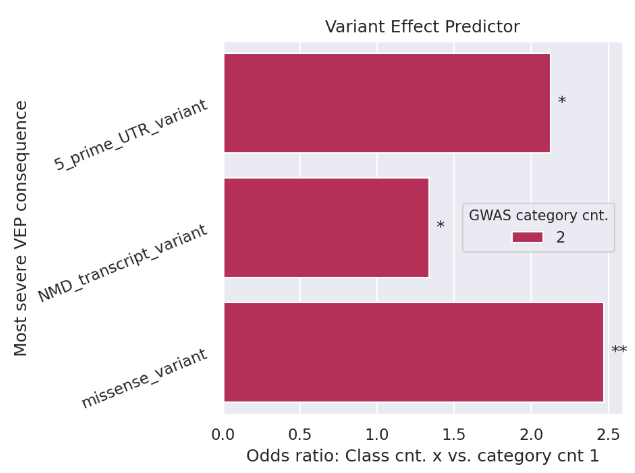
\includegraphics[width=\textwidth]{\floatRelativePath/pltbar_vep_consequence.py/vep.png}
    \end{subfigure}

    \caption{}

\end{figure}

%%%%%%%%%%%%%%%%%%%%%%%%%%%%%%%%%%%%%%%%%%%%%%%%%%%%%%%%%%%%%%%%%%%%%%%%%%%%%%%%
%
% Fig 7: Plots of the number of genes and biosample per variant-biosample and variant-gene, respectively
% Fig: TF count per GWAS class count
% Fig : eQTL gene distance
%
%%%%%%%%%%%%%%%%%%%%%%%%%%%%%%%%%%%%%%%%%%%%%%%%%%%%%%%%%%%%%%%%%%%%%%%%%%%%%%%%

\begin{figure}[!ht]

    \centering

    \begin{subfigure}[]{.49\textwidth}
        \textbf{a}
        \\
        \includegraphics[width=\textwidth]{\floatRelativePath/plt_x_per_variant_etissue_y_egene.py/plt.png}
        %
    \end{subfigure}
    %
    \begin{subfigure}[]{.49\textwidth}
        \textbf{b}
        \\
        \includegraphics[width=\textwidth]{\floatRelativePath/plt_x_per_variant_egene_y_etissue.py/plt.png}
    \end{subfigure}

%    \begin{subfigure}[]{.49\textwidth}
%        \textbf{aa}
%        \\
%        \includegraphics[width=\textwidth]{\floatRelativePath/plt_x_per_variant_etissue_y_egene.py/boxenplot.png}
%        %
%    \end{subfigure}
%    %
%    \begin{subfigure}[]{.49\textwidth}
%        \textbf{bb}
%        \\
%        \includegraphics[width=\textwidth]{\floatRelativePath/plt_x_per_variant_egene_y_etissue.py/boxenplot.png}
%    \end{subfigure}

    \begin{subfigure}[]{.49\textwidth}
        \textbf{c}
        \\
        \includegraphics[width=\textwidth]{\floatRelativePath/plt_x_per_variant_y_remapnr.py/boxenplot_custom.png}
    \end{subfigure}
    %
    \begin{subfigure}[]{.49\textwidth}
        \textbf{d}
        \\
        \includegraphics[width=\textwidth]{\floatRelativePath/plt_x_per_variant_y_remapcrm.py/remapcrm_flank10.png}
    \end{subfigure}

    \caption{}

\end{figure}

%%%%%%%%%%%%%%%%%%%%%%%%%%%%%%%%%%%%%%%%%%%%%%%%%%%%%%%%%%%%%%%%%%%%%%%%%%%%%%%%
%
% Fig: TF count per GWAS class count
% Fig : eQTL gene distance
%
%%%%%%%%%%%%%%%%%%%%%%%%%%%%%%%%%%%%%%%%%%%%%%%%%%%%%%%%%%%%%%%%%%%%%%%%%%%%%%%%

%\begin{figure}[!ht]
%    \centering
%
%    \begin{subfigure}[]{.49\textwidth}vep.png
%    \textbf{a}
%    \\
%    \includegraphics[width=\textwidth]{\floatRelativePath/plt_x_per_variant_y_remapnr.py/bxplt_remaptf_per_rsid_flank_10.png}
%    \end{subfigure}
%
%    \begin{subfigure}[]{.49\textwidth}
%        \textbf{b}
%        \\
%        \includegraphics[width=\textwidth]{\floatRelativePath/plt_x_per_variant_y_remapcrm.py/remapcrm_flank10.png}
%    \end{subfigure}
%
%    % Fig 9: eQTL gene distance
%    \begin{subfigure}[]{.49\textwidth}
%        \textbf{c}
%        \\
%        \includegraphics[width=\textwidth]{\floatRelativePath/plt_x_per_variant_y_egene_distance.py/violin.png}
%    \end{subfigure}
%
%    \caption{}
%    %
%\end{figure}

%%%%%%%%%%%%%%%%%%%%%%%%%%%%%%%%%%%%%%%%%%%%%%%%%%%%%%%%%%%%%%%%%%%%%%%%%%%%%%%%%
%%
%% Fig 9: graphical conclusions
%%
%%%%%%%%%%%%%%%%%%%%%%%%%%%%%%%%%%%%%%%%%%%%%%%%%%%%%%%%%%%%%%%%%%%%%%%%%%%%%%%%%
%
%\begin{figure}[!ht]
%    \centering
%
%    \begin{subfigure}[]{0.99\textwidth}
%        \textbf{a}
%        \\
%        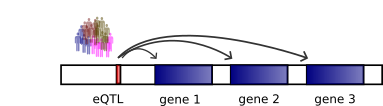
\includegraphics[width=\textwidth]{fig/model1.png}
%    \end{subfigure}
%
%\end{figure}
